\chapter[Le stage \ensg]{Le stage}

\section{Généralités}

Dans la suite de ce rapport je vais me consacrer sur les deux missions principales que j’ai réalisées à Galigeo. La première est l’estimation d’un flux piéton à une adresse donnée. (2.2) Ce n’est pas une mission réalisée pour un client en particulier, c’est une fonctionnalité qui a été ajoutée dans la dernière version des logiciels SaaS de Galigeo et est donc accessible pour tous les utilisateurs du service.

\paragraph*{}

La deuxième mission est une demande spécifique d’un client de Galigeo. J’ai eu accès à des données confidentielles à l’entreprise. Toutes les illustrations, schémas ou fragments de données, pour cette partie, seront donc fictifs

\paragraph*{}

Enfin, je terminerai rapidement sur deux autres missions clients, plus secondaires pour lesquels je rentrerai moins dans le détail.


\section{Prédiction de flux piéton}

\subsection{Mise en contexte}

Le flux piéton est une très bonne variable pour estimer le flux de consommateurs potentiels qui passe chaque jour devant une enseigne commerciale. Il est donc essentiel pour une entreprise qui fournit des services de géomarketing, de pouvoir estimer au mieux cette variable.

\paragraph*{}

Jusqu’aujourd’hui, Galigeo s’appuyait sur des estimations calculées par une autre entreprise ce qui l’empêchait de corriger les biais et erreurs possibles. Elle n’avait pas la main sur les algorithmes d’estimations.

\paragraph*{}

Ma mission a donc été de réaliser cet algorithme d’estimation du flux moyen de piéton sur une année autour d’une adresse donnée et ce pour l'ensemble du territoire national.

\paragraph{}

Il a fallu néanmoins prendre en compte les contraintes techniques de l’entreprise, les biais qui pouvaient être présents dans la donnée utilisée et l’efficacité de l’algorithme. Si les temps de calculs sont trop longs, l’expérience utilisateur risque d’être impactée mais il faut garder un modèle puissant afin de minimiser les erreurs de prédiction.

\subsection{La donnée}

Pour estimer ce flux piéton, nous allons nous appuyer sur des mesures quotidiennes que Galigeo achète à un fournisseur. En effet, Galigeo reçoit quotidiennement des positions de cellulaires sur l'ensemble du territoire métropolitain. Elle en reçoit environ 70M par mois, chacune correspondant à un évènement de visite. Cette donnée est collectée via des applications mobiles qui sont autorisées à transmettre la position du smartphone au fournisseur de Galigéo. Les positions sont anonymes mais possèdent un identifiant de smartphone ce qui permet d'avoir aussi des informations de déplacements. La donnée brute est structurée comme ci-dessous :

\begin{table}[H]
    \centering
    \begin{tabular}{|l|l|}
    \hline
    \textbf{Attribut} & \textbf{Description}              \\ \hline
    idEvent           & Id de l'évènement                 \\ \hline
    uuid              & Id du smartphone                  \\ \hline
    latitude          & Latitude de l'évènement           \\ \hline
    longitude         & Longitude de l'évènement          \\ \hline
    accuracy          & Précision de la localisation      \\ \hline
    arrival           & Date d'arrivée à la localisation  \\ \hline
    departure         & Date de départ de la localisation \\ \hline
    \end{tabular}
    \caption{Résumé de la structure d'un évènement de visite}
\end{table}

\paragraph*{}

Nous avons également utilisé de la donnée économique pour enrichir notre modèle. En effet Open Street Map propose une base open-source de POI structurée comme ci-dessous :

\begin{table}[H]
    \centering
    \begin{tabular}{|l|l|}
    \hline
    \textbf{Attribut} & \textbf{Description}                                  \\ \hline
    id\_poi           & Id du poi                                             \\ \hline
    type              & Nature du POI (Magasins, Restaurants, Epiceries, ...) \\ \hline
    latitude          & Latitude du POI                                       \\ \hline
    longitude         & Longitude du POI                                      \\ \hline
    \end{tabular}
    \caption{Structure d'un POI}
\end{table}

\paragraph*{}

Il était également intéressant de rajouter de la donnée démographique à notre modèle. Pour cela nous avons utilisé les données de population de l'INSEE agrégées au niveau des IRIS géographiques.

\paragraph*{}

Nous allons utiliser des algorithmes de Machine Learning pour estimer ce trafic piéton. Il nous faut donc des données mesurées sur le terrain afin d'entraîner un modèle. Galigeo possède plus de 11000 mesures réparties plus ou moins équitablement sur le territoire même si la plupart d'entre elles sont en milieu urbain.

\begin{figure}[H]
    \centering
    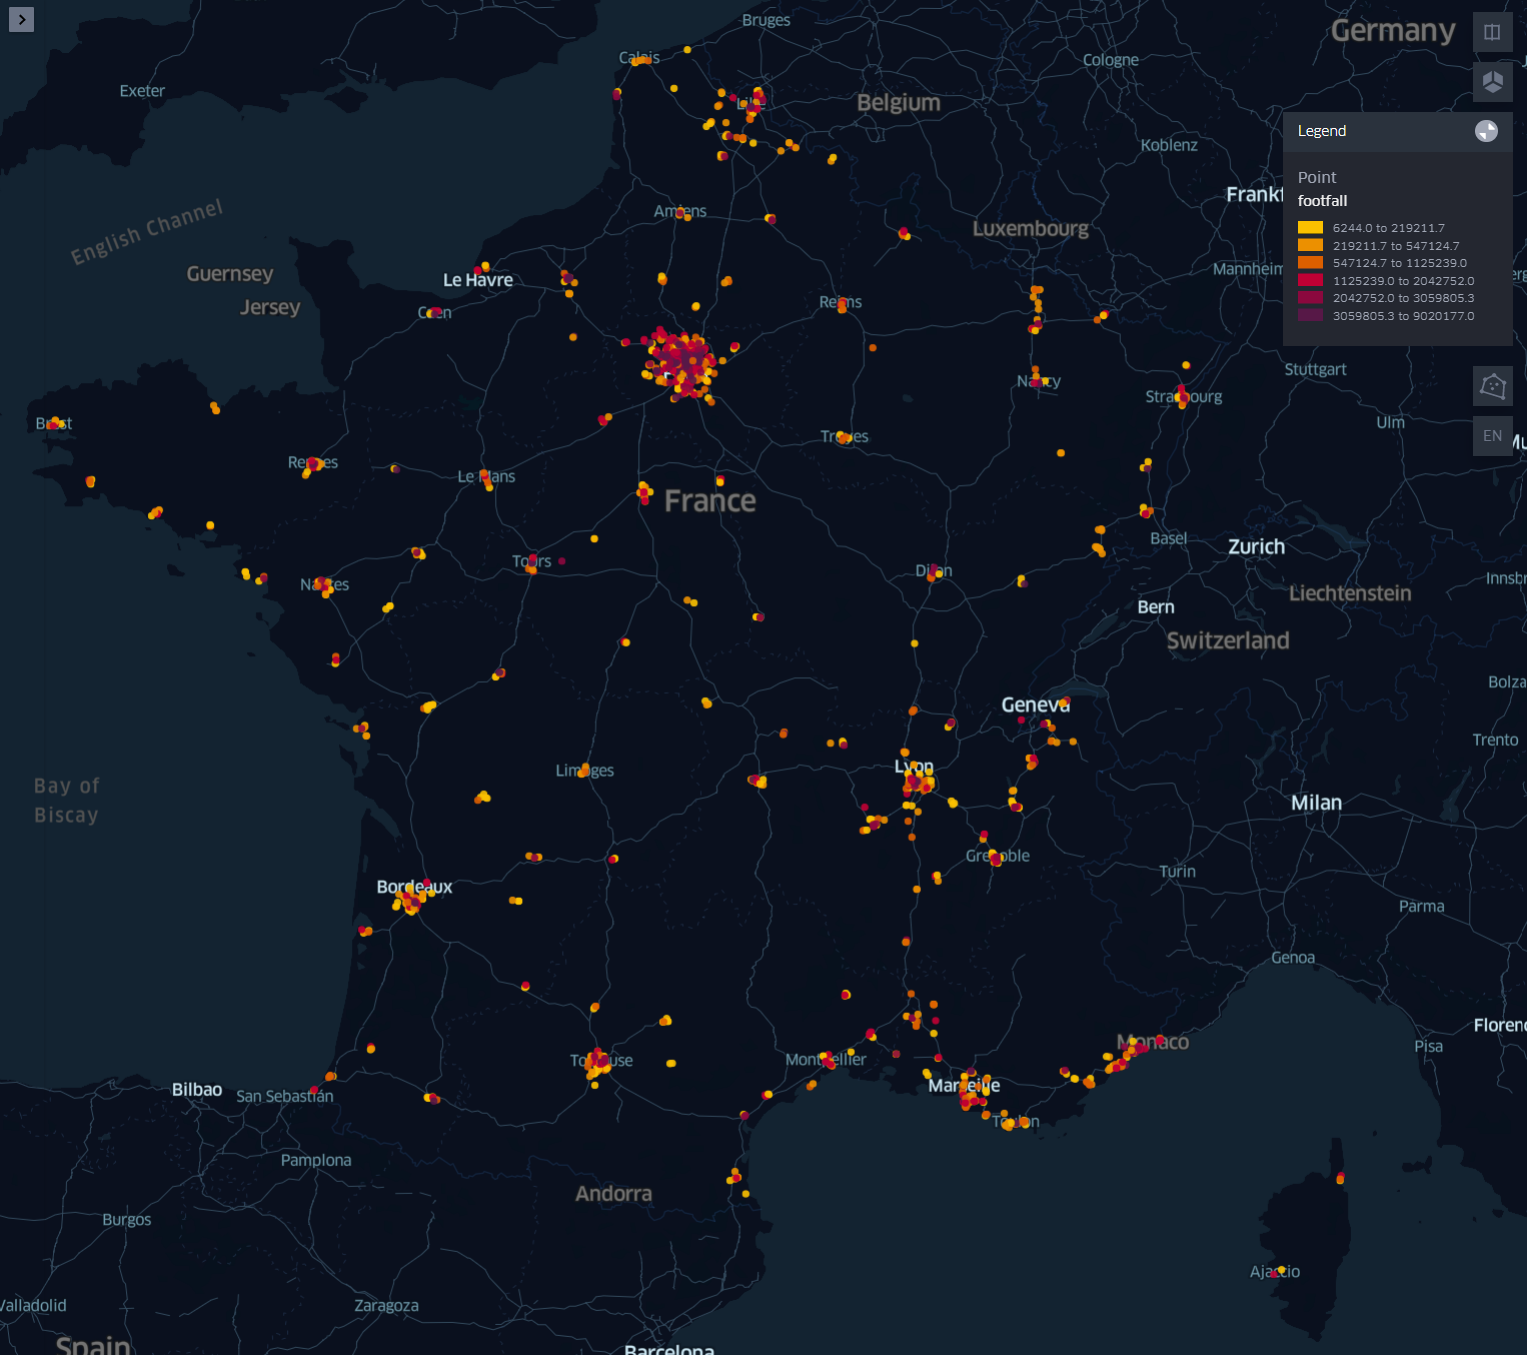
\includegraphics[width=\linewidth]{images/graphs/map_of_label_footfall.png}
    \caption{Carte des données d'entraînement}
    \label{fig:footfallmap}
\end{figure}

\subsection{Technologies utilisées}

\subsubsection{Agrégation spatiale}

Une fois que nous avons l'ensemble de nos données nous remarquons qu'elles se distinguent en deux groupes de par leur nature. Les données ponctuelles (\'Evènements de visites, POI, etc.) et les données surfaciques (Population par IRIS). Pour homogénéiser notre donnée et simplifier les futurs calculs il est important de segmenter l'espace et ajouter un index spatial à nos données.

Nous nous sommes dirigés vers la solution des hexagones H3 \cite{Uber_H3} développés par Uber. C'est un système d'indexation géospatiale qui constitue un pavage hexagonal de la sphère multi-échelles et dont les index sont hiérarchiques.

Dans notre cas c'est la solution optimale car nous pouvons l'utiliser pour joindre nos données disparates, le format hexagonal facilite la modélisation des flux et est bien adapté pour appliquer le machine learning aux données géospatiales.


% Image of the offices
\begin{figure}[H]
    \centering
    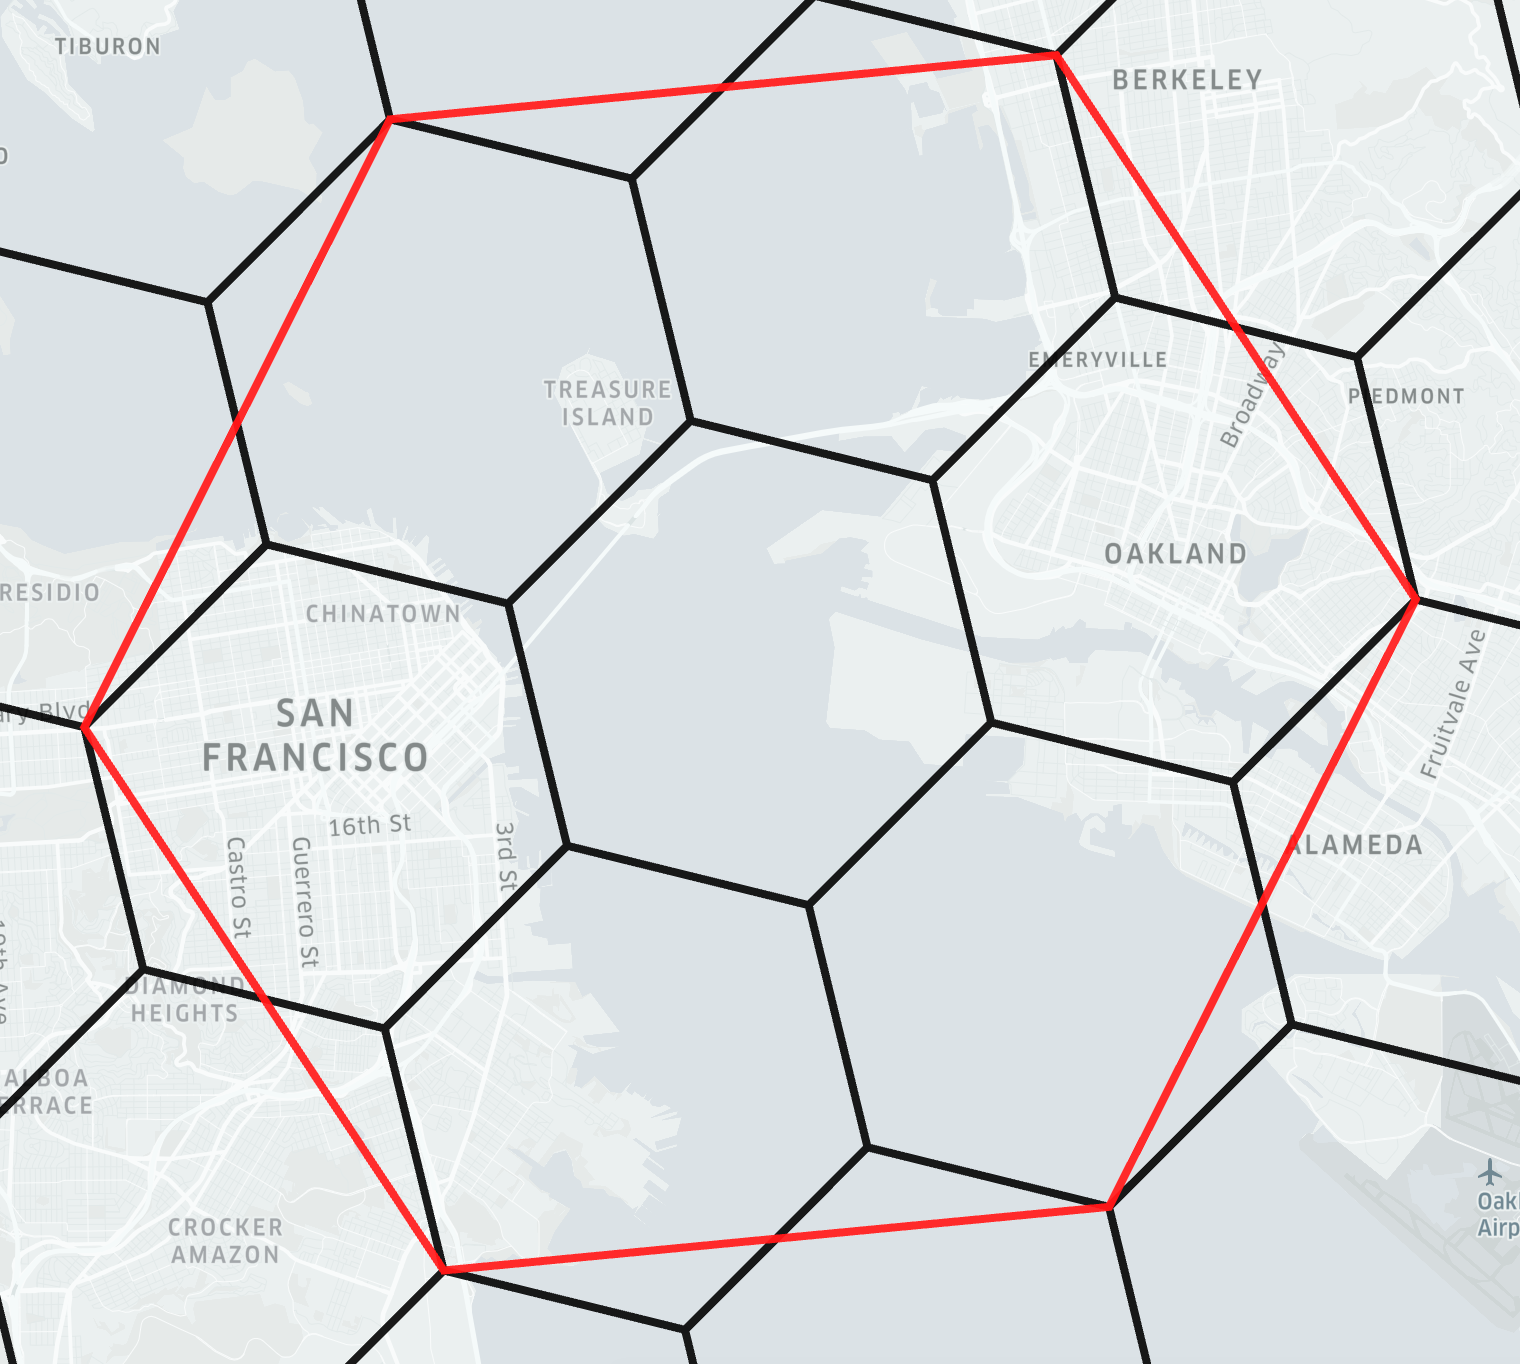
\includegraphics[width=7cm]{images/graphs/h3-multiscale.png}
    \caption{Principe de multi-echelles des cellules H3 Uber \cite{Uber_H3}}
    \label{fig:celluleh3}
\end{figure}

\begin{figure}[H]
    \centering
    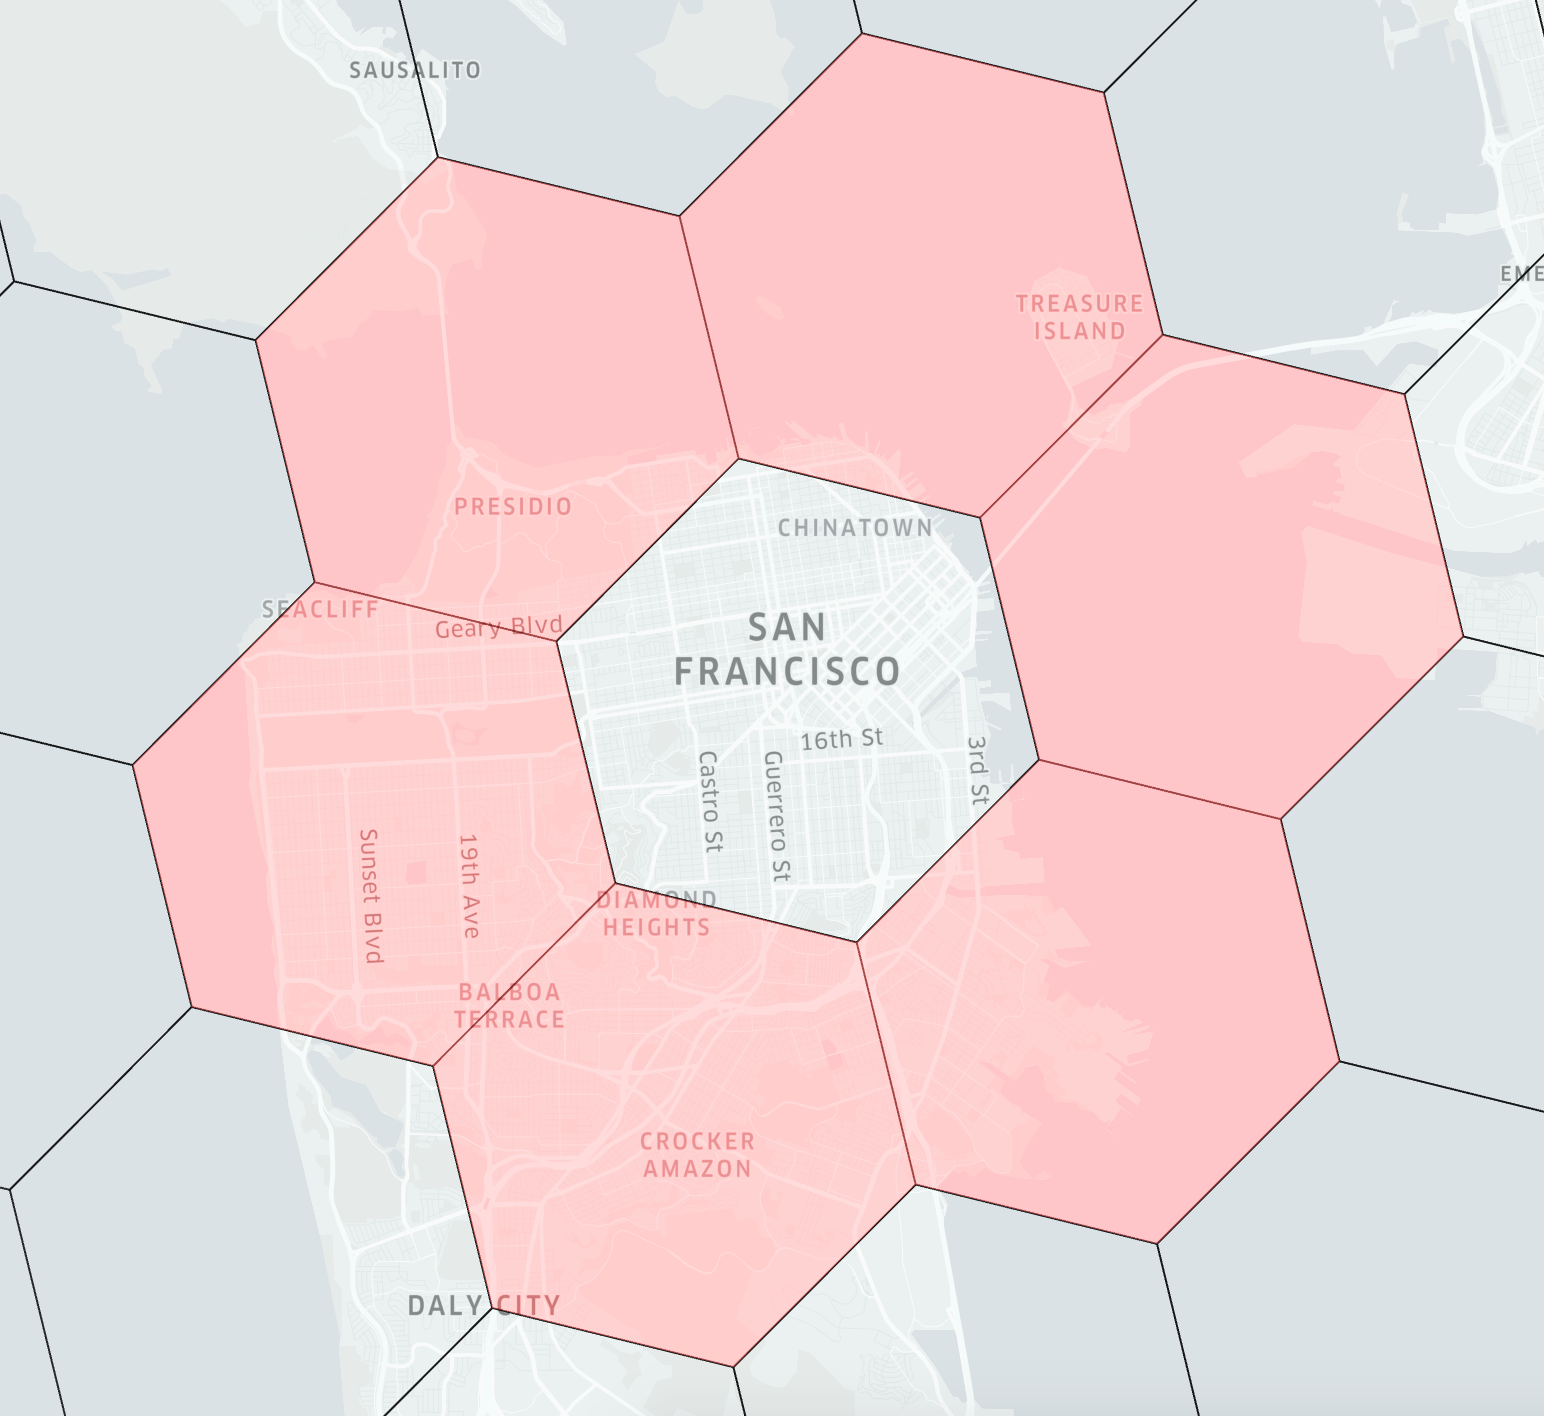
\includegraphics[width=7cm]{images/graphs/h3-ring.png}
    \captionsetup{justification=centering}
    \caption{Les 6 voisins d'une cellule H3 se rapproche d'un cercle, utile pour la modélisation de flux \cite{Uber_H3}}
    \label{fig:celluleh3ring}
\end{figure}

Pour notre part on choisira le niveau d'échelle 11, ce qui correspond environ à un hexagone de 27 mètres de rayon.

\subsubsection{Infrastructure de base de données}

Pour stocker toutes ces données, Galigeo utilise un service de Cloud Computing \footnote{Ensemble de services et de machines informatiques délocalisés dans un cloud} nommé Google Cloud Plateform (GCP) qui permet de stocker une grande quantité de données et de faire des calculs plus ou moins complexes sur celle-ci.

\paragraph*{}

Un des grands avantages de cette solution est l'intégration de Tensorflow, une bibliothèque open-source développée par Google pour faire du machine learning et de l'intelligence artificielle. Elle est très utile pour l'entraînement de réseaux de neurones profonds (DNN).

Nous pouvons également y combiner Keras, une interface open-source conçue pour simplifier l'utilisation de Tensorflow.


\subsubsection{Type de modèle utilisé}

\'Etant donnés les choix précédents, nous nous sommes donc orientés vers un modèle de Deep Neural Network (DNN).

Il est cependant important de noter que les modèles de Deep Neural Network, prouvent leur meilleure efficacité par rapport à d'autre modèles de Machine Learning lorsque la donnée est non structurée et que la taille du dataset \footnote{Tableau de données} est importante (plusieurs millions de lignes)

Dans notre cas, ces conditions ne sont pas remplies mais nous verrons plus tard dans ce rapport les alternatives envisagées.


\subsection{Préparation des données}

\subsubsection{Structuration des données}

Cette étape est cruciale pour obtenir des bons résultats après la modélisation. Il s'agit de passer de la donnée brute présentée précédemment à une donnée structurée qui permettra d'entraîner le réseau de neurones.

Pour cela, nous avons projeté l'ensemble de notre donnée brute sur la grille H3 d'Uber. Pour chaque valeur de flux piéton mesuré, nous avons calculé le nombre de visites dans la même cellule ainsi que dans les cellules voisines. Nous avons agrégé ces données events par mois sur une année complète de septembre 2021 à août 2022.

Nous avons appliqué le même principe spatial pour les POIs. Les cellules voisines se calculent très facilement grâce aux fonctions open-source mises à disposition. Ainsi on peut calculer différents anneaux autour de notre cellule de départ.


\begin{figure}[H]
    \centering
    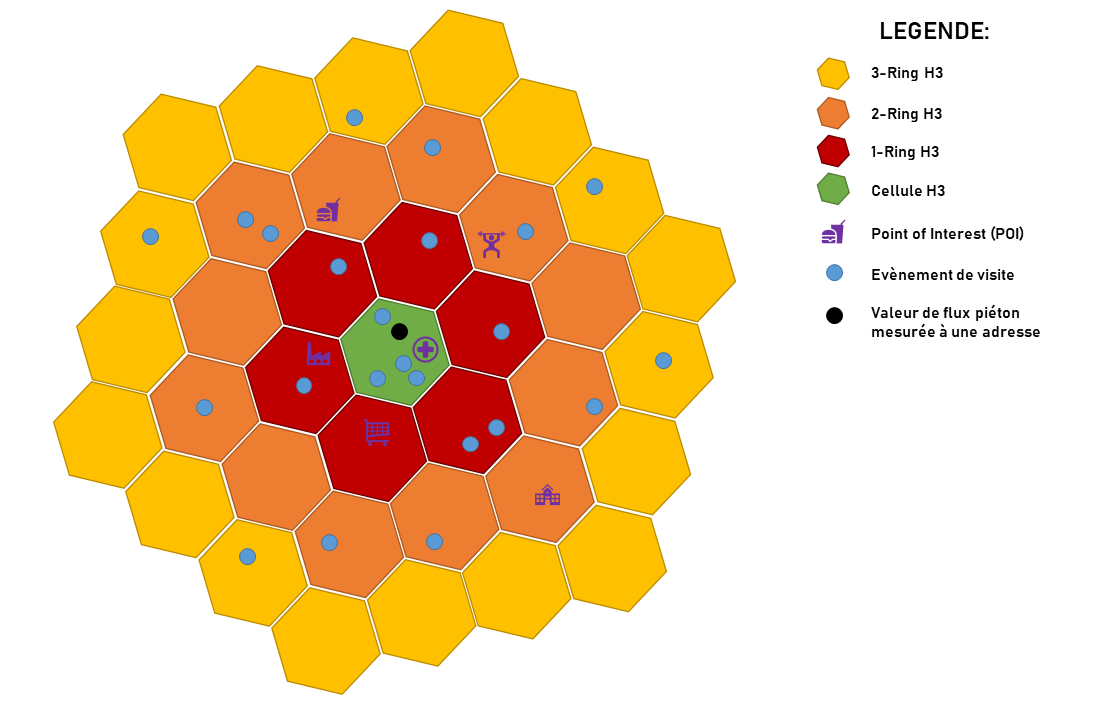
\includegraphics[width=\linewidth]{images/graphs/dataset.png}
    \captionsetup{justification=centering}
    \caption{Agrégation des données aux cellules H3 pour générer un dataset}
    \label{fig:dataset_aggregation}
\end{figure}

Pour ce qui est de la donnée de population, nous avons simplement pris le centroïde de la cellule H3, et l'avons intersecté avec les géométries des IRIS françaises afin de déterminer dans quel IRIS la cellule se trouve.

Nous avons obtenu alors une structure de dataset comme ci-dessous. Une feature est un paramètre du modèle et le label est la variable à estimer.


\begin{table}[H]
    \centering
    \begin{tabular}{|l|l|l|}
    \hline
    \textbf{Colonnes}    & \textbf{Type} & \textbf{Description}                                                    \\ \hline
    h3\_index            &               & Index de la cellule H3                                                  \\ \hline
    visits\_MMAAAA & feature       & Nb events dans la cellule H3 par mois (x12)                        \\ \hline
    visits        & feature       & Nb events dans la cellule H3 sur l'année                          \\ \hline
    visits\_k1     & feature       & Nb events dans la cellule H3 et l'anneau 1 sur l'année            \\ \hline
    visits\_k2     & feature       & Nb events dans la cellule H3 et les anneaux 1, 2 sur l'année       \\ \hline
    visits\_k3     & feature       & Nb events dans la cellule H3 et les anneaux 1, 2, 3 sur l'année    \\ \hline
    visits\_k4     & feature       & Nb events dans la cellule H3 et les anneaux 1, 2, 3, 4 sur l'année \\ \hline
    poi\_N        & feature       & Nb de POI dans la cellule H3 par nature                                 \\ \hline
    poi\_N\_k1    & feature       & Nb de POI dans l'anneau 1 par nature                   \\ \hline
    poi\_N\_k2    & feature       & Nb de POI dans les anneaux 1, 2 par nature              \\ \hline
    poi\_N\_k3    & feature       & Nb de POI dans les anneaux 1, 2, 3 par nature           \\ \hline
    poi\_N\_k4    & feature       & Nb de POI dans les anneaux 1, 2, 3, 4 par nature      \\ \hline
    population           & feature       & Population in the IRIS of the H3 cell                                   \\ \hline
    footfall             & label         & Flux piéton mesuré en un point de la cellule H3                         \\ \hline
    \end{tabular}
    \caption{Structure du dataset}
    \end{table}

On obtient alors un dataset d'environ 11000 lignes et 14 colonnes.

\subsubsection{Nettoyage des données}

La deuxième étape de la préparation des données consiste à les nettoyer pour supprimer d'abord les lignes où il manquerait certaines variables puis celles dont les valeurs du label sont aberrantes.

On se retrouve alors avec un dataset réduit de 40\%, il reste environ 6500 lignes.

\paragraph{}


Une fois ces deux étapes réalisées, nous pouvons sortir différents graphiques statistiques disponibles en annexe : KDE, Matrice de corrélation, Répartition des features.


\subsection{Tuner et Entraînement du modèle}

Notre dataset est maintenant prêt à être utilisé comme base d'apprentissage. Nous avons donc créé une structure de modèle. Cette structure possède des paramètres appelés Hyperparamètres. Chaque hyperparamètre peut prendre une valeur parmi une liste bien définie. Le principe du Tuner est de compiler ce modèle plusieurs fois avec des valeurs d'hyperparamètres bien différentes et choisies aléatoirement.

\begin{figure}[H]
    \centering
    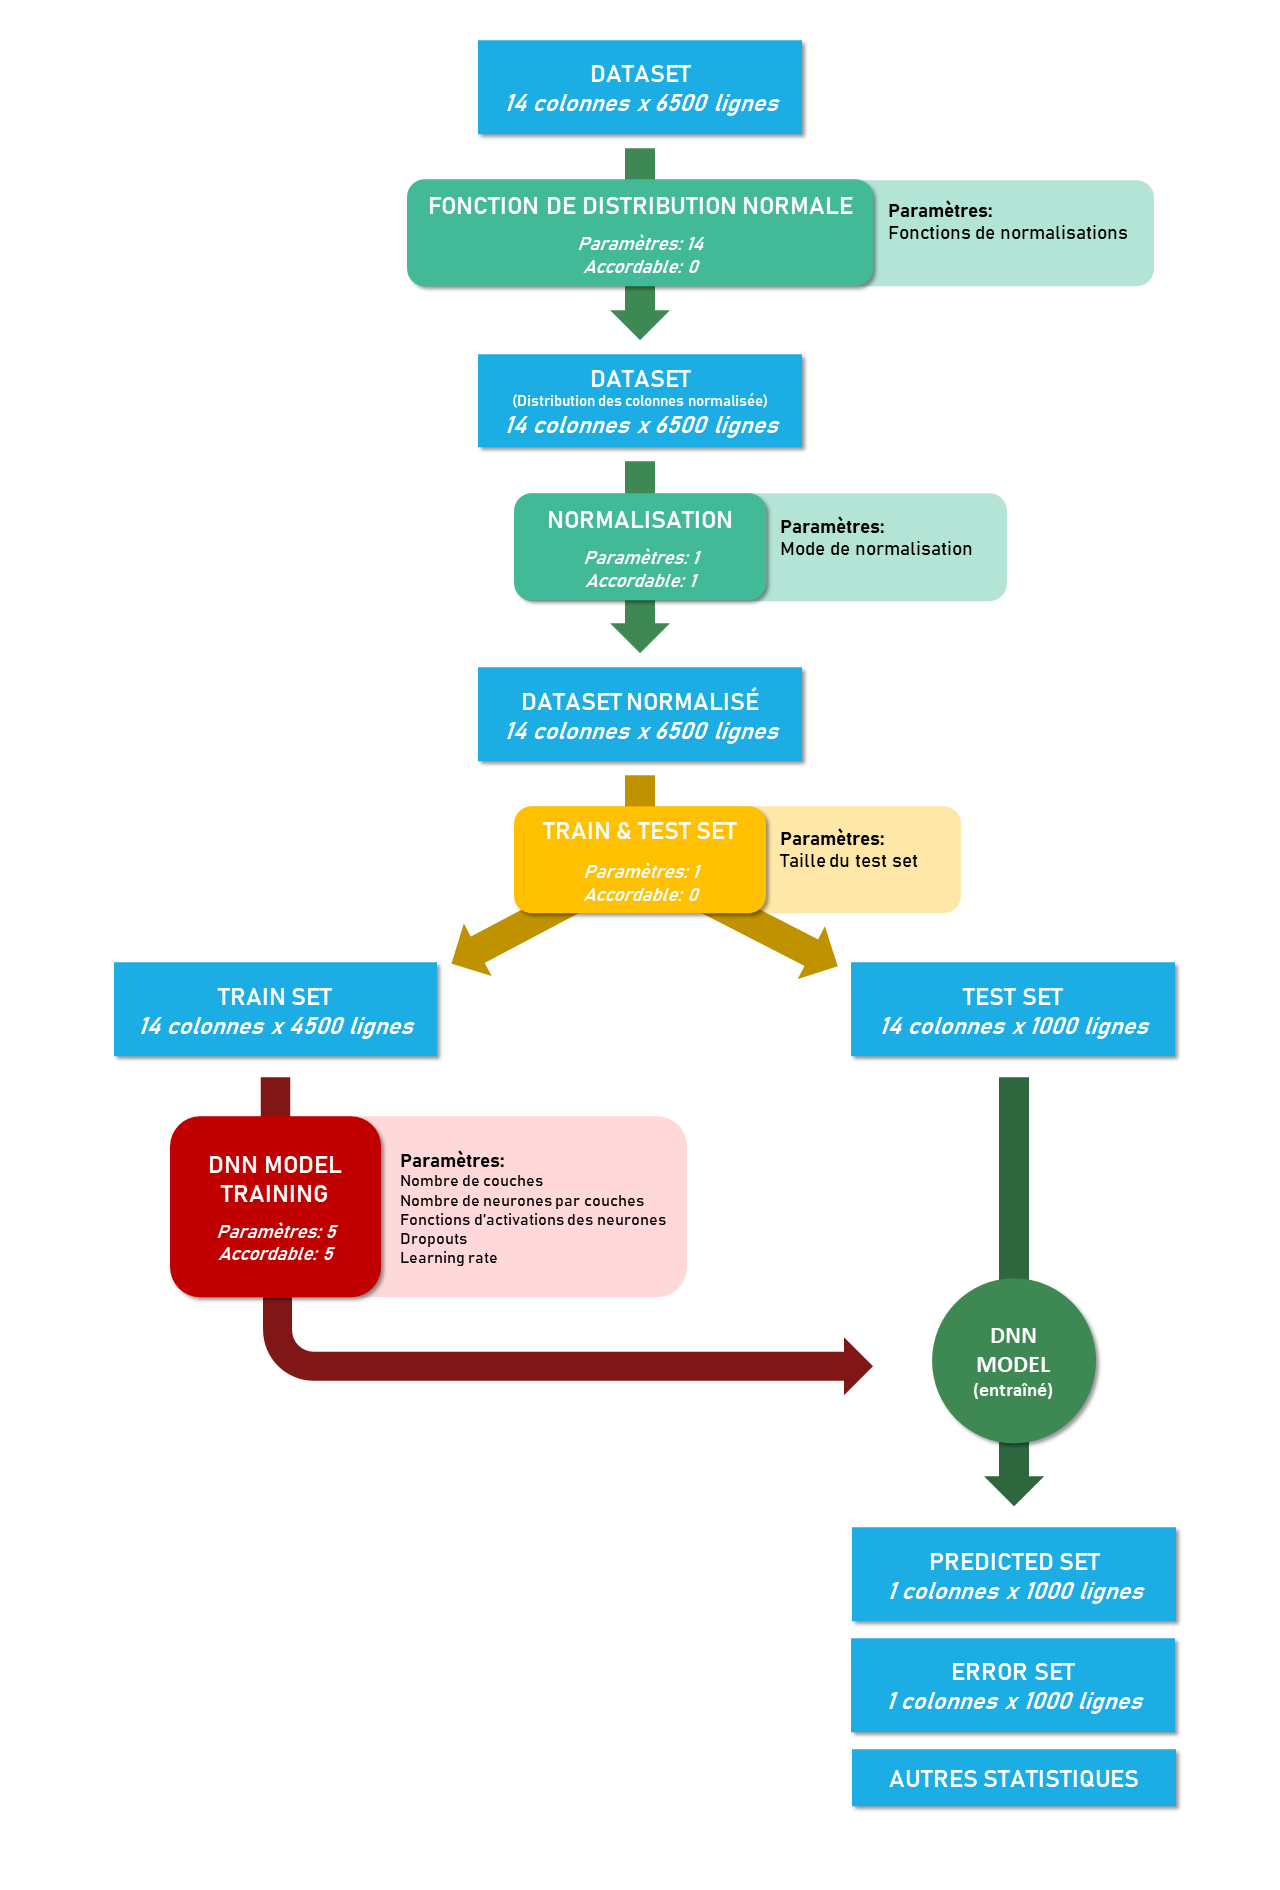
\includegraphics[width=\linewidth]{images/graphs/struc_model_dnn.png}
    \captionsetup{justification=centering}
    \caption{Structure du modèle envisagé}
    \label{fig:strcu_dnn}
\end{figure}

La première étape de notre modèle est donc de normaliser la distribution de nos features /footnote{Paramètres d'entrée du modèle}. En effet, la distribution des valeurs pour chaque features n'est pas forcément "normale" et il est préférable de passer nos valeurs à travers une fonction pour la modifier.

\begin{figure}[H]
    \centering
    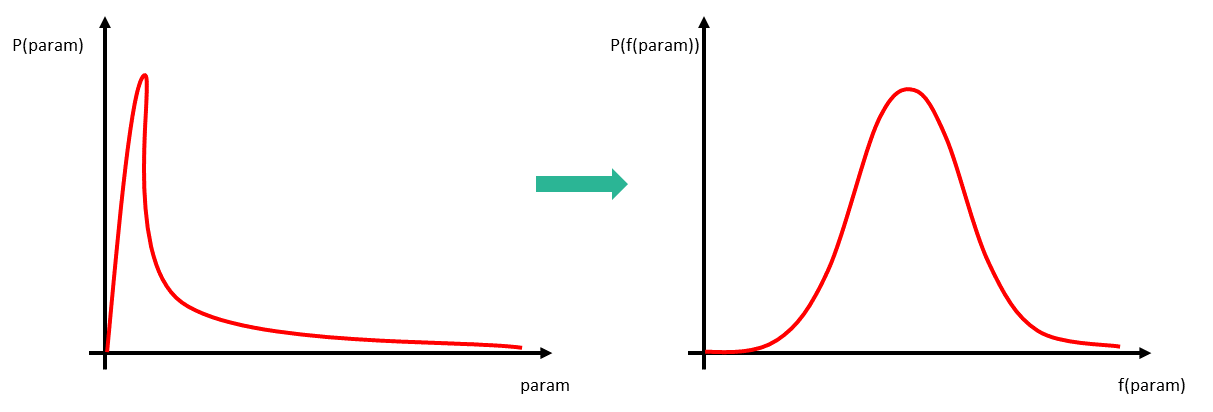
\includegraphics[width=\linewidth]{images/graphs/fct_histo.png}
    \captionsetup{justification=centering}
    \caption{Principe de normalisation de la distribution d'une feature}
    \label{fig:fct_repartition}
\end{figure}

L'étape suivante est de normaliser les valeurs de nos features (cette fois ci, on ne modifie pas le label \footnote{Variable estimé en sortie du modèle}). Pour cela, il existe principalement deux types de normalisation : La normalisation min/max et la normalisation moyenne/écart-type.

Cela permet entre autre d'assurer une cohérence entre les données et permet à l'exécution d'être plus rapide et meilleure.


\paragraph{}

Une fois cette étape réalisée, nous divisons en deux parties aléatoires (la proportion est contrôlée) le dataset normalisé. La partie "trainset" permet d'entraîner le modèle et la partie "testset" permet de vérifier si le modèle est correctement entraîné.

\paragraph{}

L'objectif est maintenant d'obtenir un réseau de neurones entraîné. Pour cela, nous utilisons un modèle construit sur les hyperparamètres et lui passons l'ensemble du trainset en entrée. En parcourant l'ensemble des données et en essayant d'estimer le label, le réseau de neurone apprend et règle ses paramètres internes (poids des axones, valeur interne des neurones, etc.) en appliquant une validation croisée.

De cette étape, nous récupérons un réseau de neurones profonds qui permet maintenant d'estimer notre label en fonction de nos features.


\paragraph{}

Nous passons donc notre testset dans notre réseau neuronal. Cela nous permet d'obtenir notre label estimé et de le comparer au vrai label. On obtient alors une liste de n erreurs (dans notre cas 1000), grâce auxquels nous pouvons mesurer la qualité du réseau de neurones. On peut calculer l'erreur quadratique moyenne (RMSE), un coefficient de détermination (R2) ou la précision du modèle ("accuracy").

\subsection{Résultats}

\begin{table}[H]
    \centering
    \begin{tabular}{l|l|l|}
    \cline{2-3}
                                            & \textbf{Test set} & \textbf{Training set} \\ \hline
    \multicolumn{1}{|l|}{\textbf{RMSE}}     & 1 000 000         & 500 000                \\ \hline
    \multicolumn{1}{|l|}{\textbf{R2 Score}} & 0.45              & 0.86                  \\ \hline
    \end{tabular}
    \caption{Résumé des résultats}
\end{table}

Pour estimer la qualité de notre modèle, il faut regarder les résultats de la colonne de gauche, "Test set". On remarque tout de suite que l’erreur moyenne quadratique est d’environ 1000000. Or, si l’on se réfère à l’annexe B, Statistiques du modèle, on remarque que le flux piéton médian est de 1000000 également.

Le R2 score est également faible. Idéalement, il devrait se rapprocher de 1. L’estimation que fait le modèle n’est donc pas encore suffisante. 

\paragraph*{}

Cependant Galigeo renforce son dataset à chaque arrivée de données ce qui peut améliorer les résultats par la suite. Il se peut également que 6500 entrées soit trop peu et que l’enrichissement de mesure permette également de rendre plus précises les estimations du modèle.

Nous avons également discuté de nombreuses autres pistes pour obtenir des résultats plus intéressant mais je les détaillerai dans la partie 3.1 de ce rapport.

\section{Prédiction de chiffre d'affaire}

\subsection{Contexte}

Pour qu’une entreprise continue à croître et à se développer, elle peut étendre son aire d’attraction et ainsi cibler plus de clients. L’entreprise décide alors d’ouvrir une nouvelle enseigne. Le choix de l’emplacement est alors stratégique.

Pour ce projet, un client de Galigeo souhaite implanter de nouvelles enseignes sur le territoire français. Pour ce faire il souhaite estimer le chiffre d’affaires qu’engendrerait un magasin en fonction de sa localisation, de sa surface, du type de magasin et du flux piéton moyen à l’adresse. 

\paragraph{}

Il a donc fallu créer un modèle prédictif du chiffre d’affaires en s’entraînant sur les données des enseignes existantes. Cependant, cette entreprise possède 150 enseignes environ en France et cela semble insuffisant pour entraîner un modèle de machine learning. Nous avons donc utilisé une autre méthode pour démultiplier les données.


\subsection{Données}

La France est découpée en 15 500 IRIS (îlots Regroupés pour l'Information Statistique) et le client possède des données commerciales pour certains d’entre eux. Il est alors intéressant de travailler sur les IRIS et non sur les enseignes. En effet, nous avons à disposition :

\begin{itemize}
    \item La liste des enseignes (surface, chiffre d’affaires, type, localisation, …)
    \item La liste des concurrents (surface, type, localisation, …)
    \item Des données socio-démographiques pour chaque IRIS (tranche d’âge, nombre de ménage, revenue moyen, …)
    \item Un distancier des Iris (permet de connaitre la distance et le temps de parcours entre deux centroïdes d’Iris)
    \item Une estimation de la valeur du marché dans chaque IRIS
    \item Une valeur de chiffre d’affaires pour chaque enseigne dans chaque IRIS (C’est ici le chiffre d’affaires tracé, une partie du chiffre d’affaires de chaque enseigne ne peut pas être localisée)
\end{itemize}

\paragraph{}

On peut alors créer un dataset où chaque élément correspond à un IRIS pour un magasin et agréger le reste de la donnée à cette structure. On cherchera alors à estimer une part de marché, qui correspond à la quantité de marché détenu par un magasin particulier. Chaque enseigne connait l'origine géographique d'une partie de son chiffre d'affaire (~20\%), on peut donc connaitre cette part de marché sous-évaluée, en divisant ce chiffre d'affaire tracé par la valeur du marché dans un IRIS donnée.

\begin{figure}[H]
    \centering
    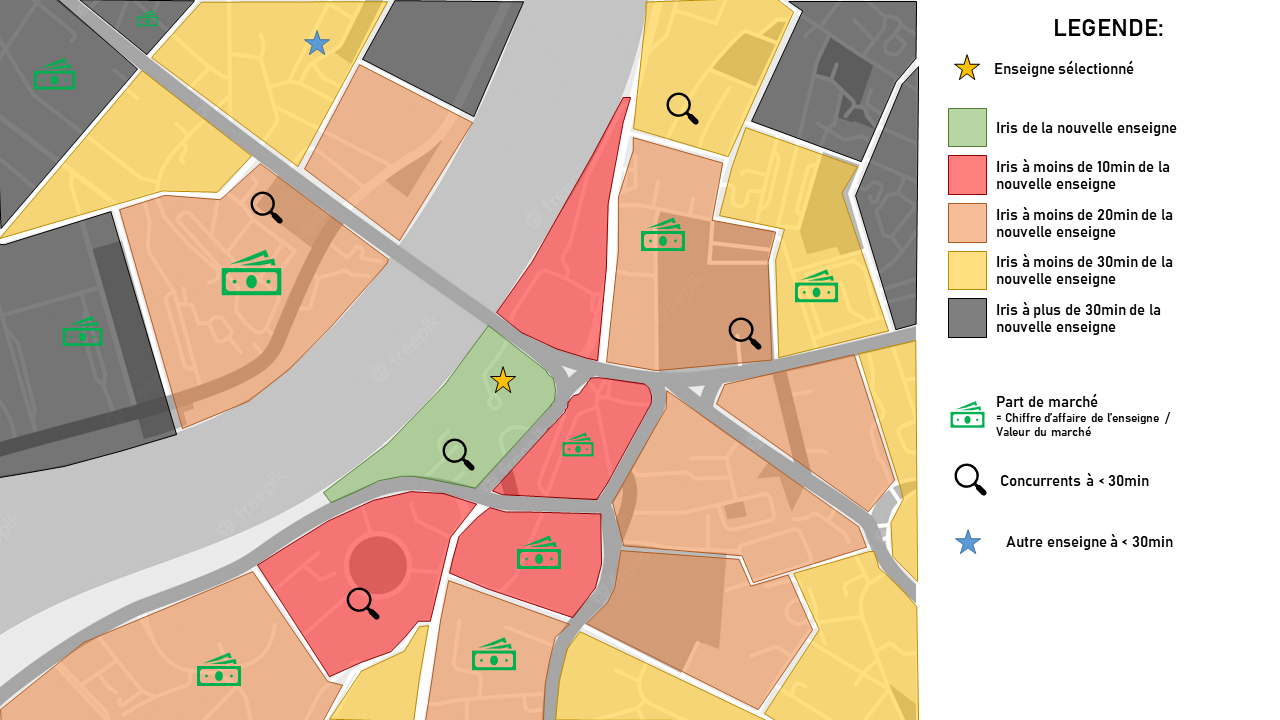
\includegraphics[width=\linewidth]{images/graphs/data_ca.png}
    \captionsetup{justification=centering}
    \caption{Résumé de l'agrégation des données}
    \label{fig:data_ca}
\end{figure}

\subsection{Structure du modèle}

Cette fois-ci, il était plus intéressant de ne pas choisir un algorithme de Deep Learning mais un algorithme de machine learning moins coûteux en ressource comme un régresseur « Random Forest » ou un « XGBoost ».
On utilisera la même structure de modèle qu’à la partie 2.2 mais cette fois-ci la normalisation est moins importante car le modèle n’est pas composé de neurones mais d’arbres de décisions.
Nous avons donc,cette fois-ci, fait deux fois la manipulation: une fois avec un régresseur XGBoost et une fois avec  un régresseur RandomForest pour choisir le modèle le mieux approprié.


\subsection{Résultats}

Grâce à nos deux modèles, nous avons pu faire des prédictions et les comparer:


\begin{figure}[H]
    \centering
    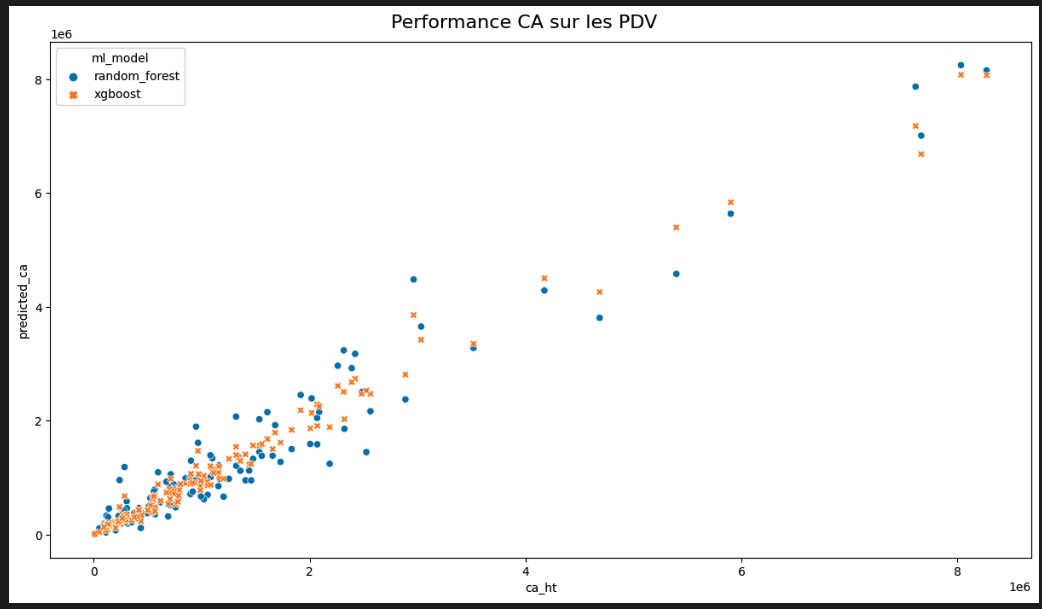
\includegraphics[width=13cm]{images/graphs/result_ca.png}
    \captionsetup{justification=centering}
    \caption{Résultat: Prédiction en fonction des mesures}
    \label{fig:result_ca}
\end{figure}

Nous avons donc choisi d'utiliser le modèle XGBoost qui nous permet d'avoir des prédiction beaucoup plus fiable.

\'A l'heure actuelle, nous attendons une réunion avec le client afin de vérifier que nos résultats concordent avec les leurs.

\section{Autres missions}

\subsection{Analyse de données - Base de données nationale des Bâtiments}

Pendant mon stage, j’ai également pu travailler sur d’autres petites missions pour des clients de Galigeo pour lesquels il n’était pas forcément question de machine learning.

\paragraph{}

Un client de Galigeo réalise de la prospection chez des particuliers. Jusqu’ici, la prospection était organisée très simplement, un quartier était sélectionné et les prospecteurs passaient dans chaque habitation. Ce client cible les habitations se chauffant à l’électricité et il arrive souvent que certaines des habitations prospectées se chauffent au gaz ou autre. Dans un souci d’économie et de gain de temps, nous avons donc tenté de cibler les prospections.

En janvier 2022, une Base de Données Nationale des Bâtiments \cite{BDNB} est mise en ligne en open-source. C’est une base très complète avec plus de 90\% des géométries renseignés. Environ 25\% des bâtiments possèdent des informations énergétiques dont on ne connait pas la qualité. Le client et Galigeo ont donc décidé de mener une campagne de prospections cet été en s’appuyant sur cette base de données afin de qualifier les données énergétiques disponibles. Nous avons donc fait de l’analyse de données sur quelques IRIS (à Rennes et à Paris) pour lancer la campagne de prospection.

\paragraph{}

Aujourd’hui les campagnes de prospections sont toujours en cours mais le résultat semble positif. Si la base de données est retenue pour diriger les campagnes de prospections du client, il faudra automatiser les processus d’analyse pour envoyer la donnée traitée dans leur application métier développée par Galigeo.

Sachant que seulement 25\% des bâtiments ont des données énergétiques, il sera peut-être intéressant un jour d’utiliser un algorithme de classification par machine learning pour interpoler ces informations manquantes sur le reste de la base. 


\subsection{Data engineering - Scrapping et automatisation de chaîne d'acquisition de données}

Une autre mission que j’ai pu réaliser était pour un client international de Galigeo. Ils utilisaient la solution de Galigeo pour leurs compagnies en France et souhaitent l’utiliser dans 13 nouveaux pays. La solution actuelle permet de sortir des rapports de géomarketing poussés qui s’appuient sur de très grandes quantités de données.

L’objectif était donc de récupérer de la donnée en quantité et d’automatiser son processus de publication dans une base de données. J’ai donc écrit des scripts permettant de scrapper des sites web de concurrents pour récupérer de la donnée non structurée pour l’organiser. J’ai aussi dû automatiser des requêtes via des API afin de récupérer des données ponctuelles sur un pays entier.

\paragraph*{}

Ce projet est encore en cours à la date où je rédige ce rapport. L’application et la base de données complète devrait être livrée pour la mi-octobre.
